

\section{Диаграммы цвет-интенсивность}

Если построить диаграмму цвет-интенсивность \ref{fig:color-magnitude}, то можно увидеть, насколько отличается блеск кандидатов от блеска остальных источников в области и от эталонной выборки. Видно, что звёзды выборки гораздо ярче как кандидатов, так и всех звёзд области. 

Большинство кандидатов очень слабые, их звёздные величины находятся на грани чувствительности GALEX. Также видно, что цвет FUV-NUV у кандидатов может быть отрицательным, и также просто отличаться от эталонных. Это даёт представление о количестве кандидатов, пришедших в выборку с третьим, неультрафиолетовым критерием.

Источников на рисунке \ref{fig:color-magnitude} меньше, чем в итоговом списке, так как многие как кандидаты, так и остальные звёзды не имеют FUV измерений.

\begin{figure}[ht]
\center{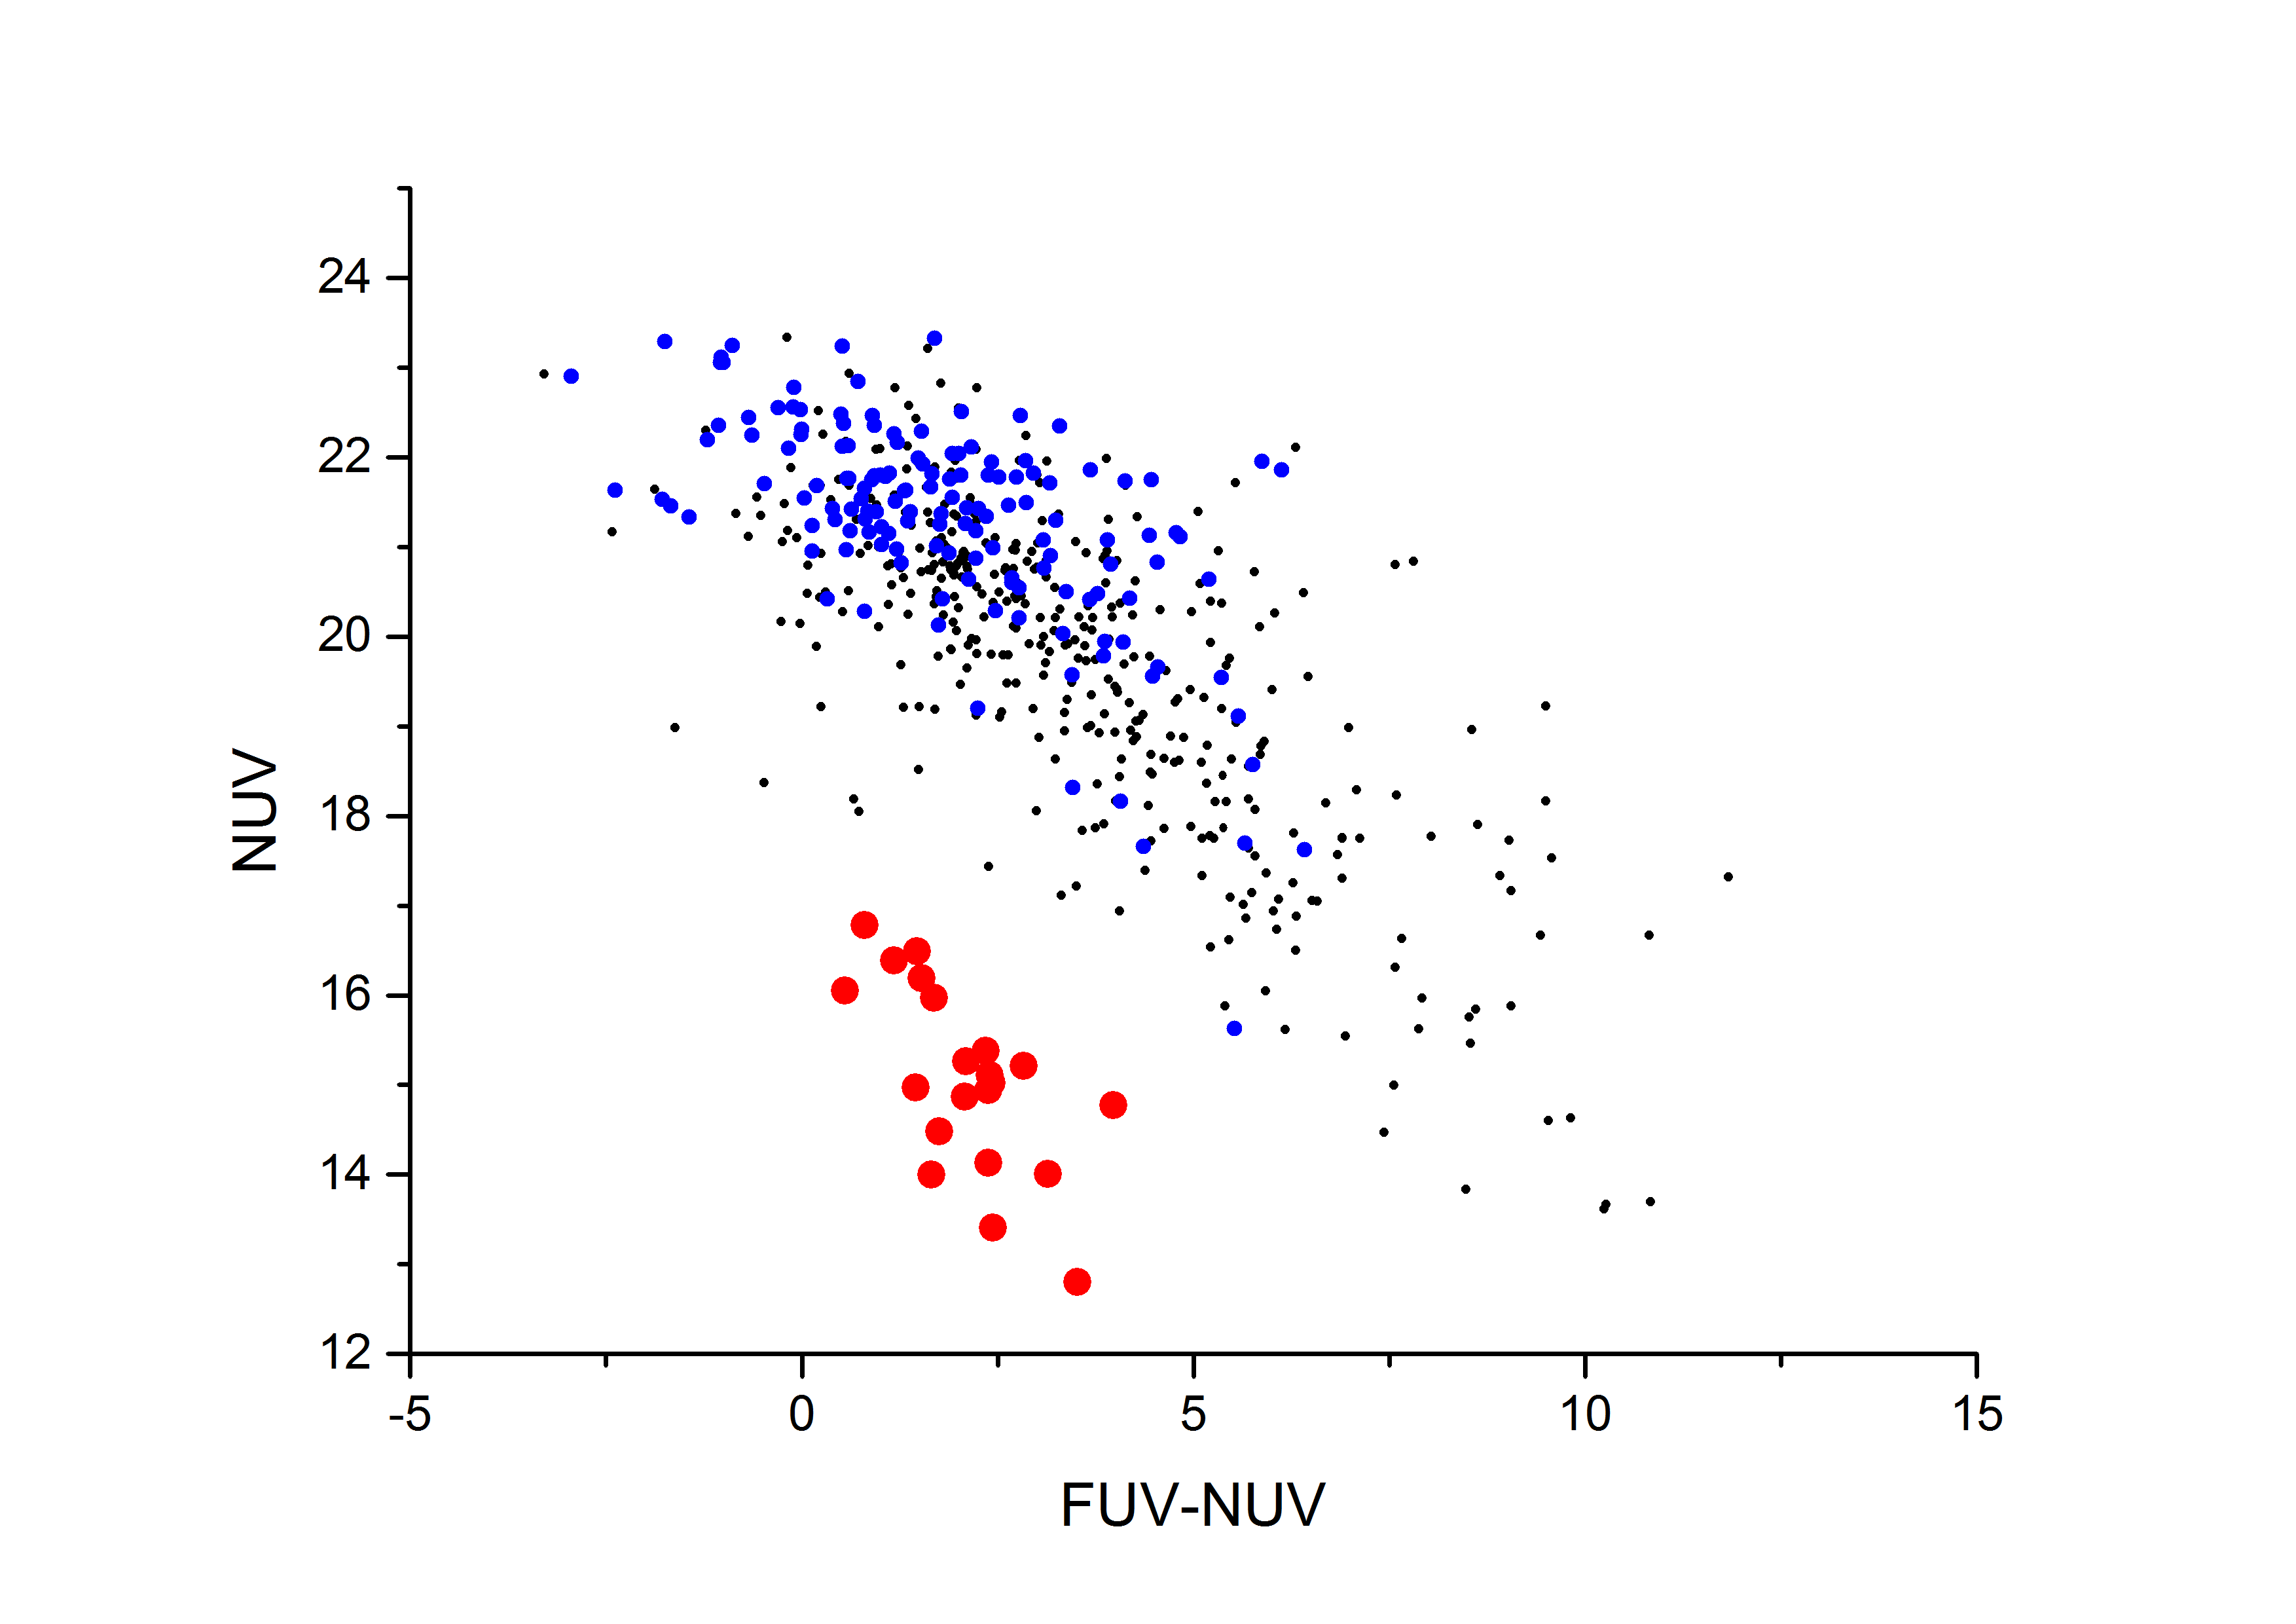
\includegraphics[width=0.6\linewidth]{colormagnitude.png}}
\hfill
\caption{Диаграмма цвет-интенсивность. Красным отмечены звёзды эталонной выборки, синим -- отобранные кандидаты}
\label{fig:color-magnitude}
\end{figure}

\section{Распределение спектральной энергии}

Сервис VOSA, использовавшийся для оценки эффективных температур, может строить распределение спектральной энергии, SED. Мы можем построить такую характеристику для эталонных звёзд, например, для T Tau, которая также входит в этот список, и сравнить с ней SED кандидатов. 

Как видно из рисунка, распределения не всегда похожи. Однако у большинства кандидатов в ультрафиолетовом диапазоне присутствует пик, подобный пику у T Tau.

\begin{figure}[ht]
\begin{minipage}[ht]{0.49\linewidth}
\center{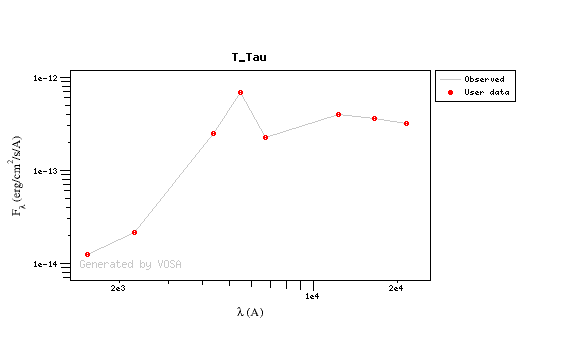
\includegraphics[width=1\linewidth]{T_Tau.png} \\ }
\end{minipage}
\hfill
\begin{minipage}[ht]{0.49\linewidth}
\center{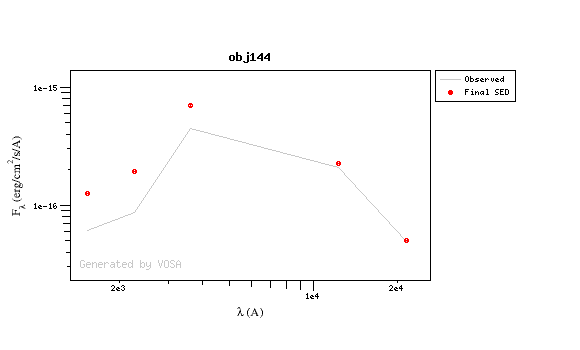
\includegraphics[width=1\linewidth]{obj144.png} \\ }
\end{minipage}
\begin{minipage}[ht]{0.49\linewidth}
\center{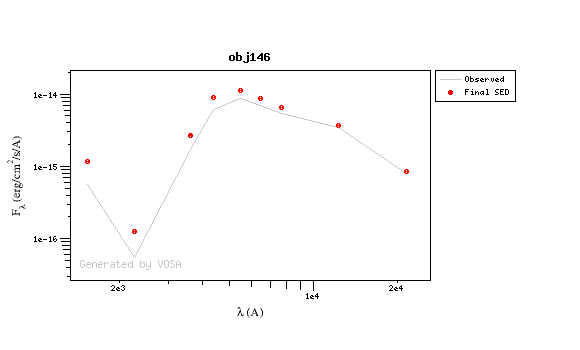
\includegraphics[width=1\linewidth]{obj146.png} \\ }
\end{minipage}
\hfill
\begin{minipage}[ht]{0.49\linewidth}
\center{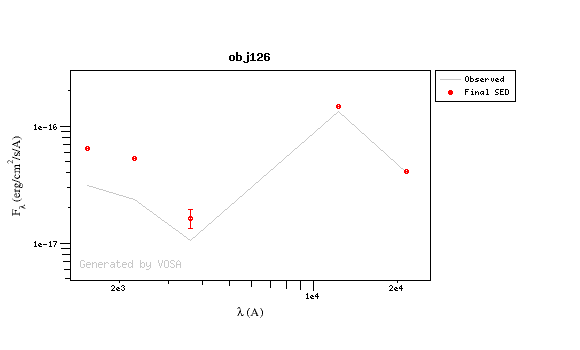
\includegraphics[width=1\linewidth]{obj126.png} \\ }
\end{minipage}
\caption{Распределение спектральной энергии (SED) для T Tau и некоторых из кандидатов}
\label{fig:sed}
\end{figure}

\section{Оценка поглощения}

Межзвёздное поглощение в исследуемой области определяется в основном наличием молекулярных облаков. Однако, наблюдения миссии GALEX относятся только к периферии этих облаков, где поглощение значительно ниже. По некоторым оценкам, его величина $A_v < 0.5$ \cite{AIGdC2014galex} по другим $A_v < 0.5$ \cite{park2012far}, и таким поглощением можно пренебречь.

\section{Расположение}
Картинки с координатами и собственными движениями.

\section{Классические и со слабыми линиями}
В соответствии с результатами, полученными в аналогичном исследовании \cite{AIGdC2014galex}, WTTS и CTTS также находятся в разных областях двухцветной диаграммы FUV-NUV vs J-K:
\begin{itemize}
	\item Положение WTTS определяется линией $FUV - NUV = -(3.88 \pm 0.61)(J - K) + (5.64 \pm 0.55)$, среднеквадратичное отклонение равно 0.59.
	\item CTTS имеют нормальное распределение по оси $J - K$ со средним значением $a = 1.4$ и дисперсией $\sigma = 0.4$. По оси $FUV - NUV$ они распределены равномерно.
\end{itemize}

\begin{figure}[ht]
\center{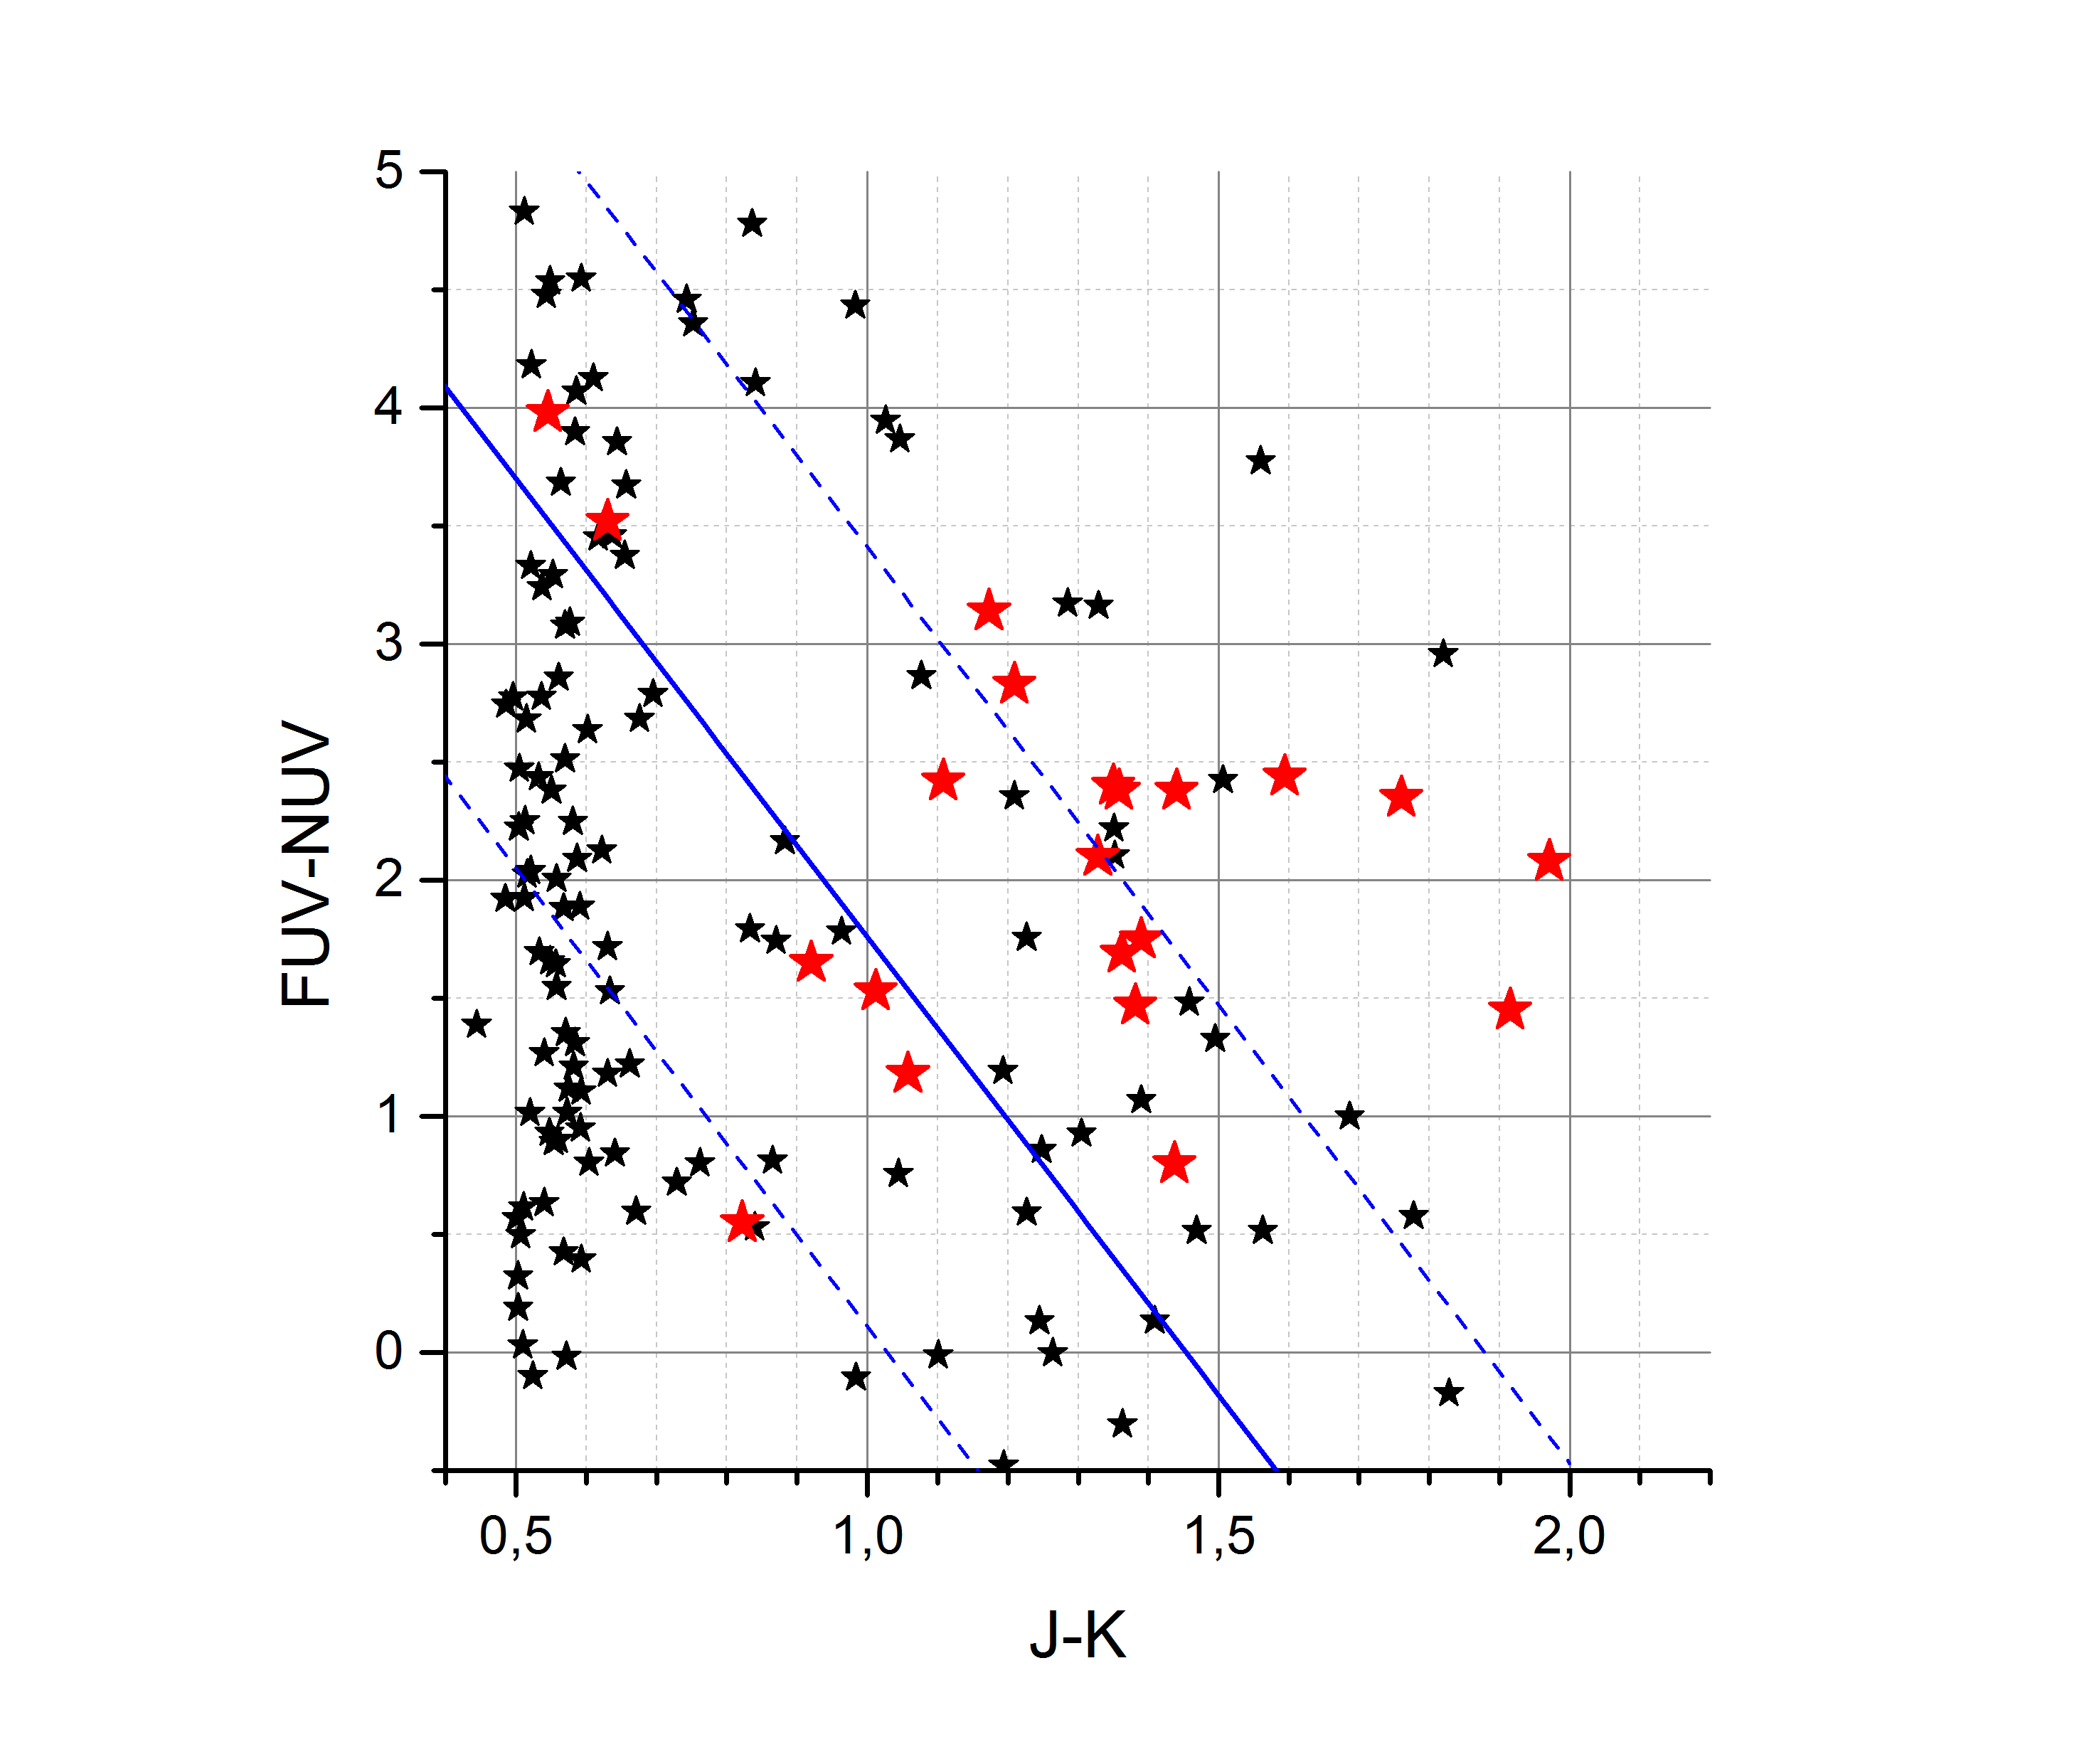
\includegraphics[width=0.6\linewidth]{trend.png}}
\hfill
\caption{Двухцветная диаграмма FUV - NUV vs J - K. Красным обозначены звёзды эталонной выборки, чёрным -- кандидаты. Синими прямыми выделена область, в которой расположены WTTS.}
\label{fig:trend}
\end{figure}

Теперь можно распределить кандидаты в группы согласно этим результатам. К звёздам типа Т Тельца со слабыми линиями относим те, что лежат между штриховыми прямыми на рисунке \ref{fig:trend} (границы взяты втрое шире, чем коридор ошибок приближения), и имеют FUV~-~NUV > 3.5. К классическим T Tauri отнесём источники, у которых 0 < FUV~-~NUV < 3.5. Остальные кандидаты, включая не имеющие FUV, будем считать кандидатами в T Tauri звёзды без более детальной классификации.



